% ---------------------------------------------------------------------
% IV. RESULTS (about 1 page)
% Owners: Julia and Bláithín
%
% FIRST DRAFT (2026-10-21): what goes where + numbers and
% source CSVs. Report results only; interpretation
% goes in Section V. 
% ---------------------------------------------------------------------
\section{Results}\label{sec:results}

\todo{Rough first draft: plan bullets with numbers, to be turned into prose.}

\subsection{What the Explainers Say}
% Exp 1 (Bláithín). Sources: exp1_summary.csv, exp1_results.csv.
In Experiment~1, the original model still scored 7 of the 16 report sentences above 0.5,
along with 9 of the 16 counter-speech sentences and 15 of the 16 promoting ones.
Mean toxicity was 0.88 for promote, 0.43 for report and 0.57 for counter sentences
(0.96, 0.84 and 0.74 for the unbiased model). SHAP put on average 87\% of the toward-toxic 
attribution in report sentences on the insult words, compared with 75\% for promote and 69\% for counter sentences.

\begin{itemize}
  \item 3--4 sentences recapping Exp 1 and Exp 2. No figure.
  \item Exp 2: harmless identity sentences score far above control sentences; SHAP puts the decision on the identity word (\texttt{exp2\_results.csv}).
  \item SHAP and LIME agree on the top word in 78/88 sentences.
  \item ``But are these explanations faithful?''
\end{itemize}

\subsection{Faithfulness to the References}
\begin{itemize}
  \item Fig.~\ref{fig:cf} and Table~\ref{tab:faith} go here.
  \item Exp 3, SHAP vs.\ counterfactual (\texttt{exp3\_faithfulness\_shap.csv}): sentence level ($n=150$) $\rho = 0.96$ (original) / 0.92 (unbiased), sign agreement 0.98 / 0.93, MAE 0.94 / 0.72 log-odds. Term level ($n=15$) $\rho = 0.98$ / 0.95.
  \item Exp 3, LIME vs.\ counterfactual (\texttt{exp3\_faithfulness\_lime.csv}): $\rho = 0.97$ / 0.97, sign agreement 0.99. LIME's MAE (0.07 / 0.04) is on the \textbf{probability} scale (\texttt{cf\_p\_*}, \texttt{est\_lime\_*} columns), so don't compare it with SHAP's log-odds MAE.
  \item The 46\% $\rightarrow$ 60\% re-test (\texttt{exp3\_debias\_retest.csv}): share of $|$SHAP$|$ 46\% $\rightarrow$ 60\%; counterfactual effect 3.36 $\rightarrow$ 3.60 log-odds; SHAP estimate 4.16 $\rightarrow$ 3.84. Say plainly how much of the claim survives.
\end{itemize}

% Exp 4 (Bláithín). Sources: exp4_auc.csv, exp4_summary.csv,
% exp4_identity_coefs.csv; median rho, 96% and 4% from the EXP4 run notes.
On the transparent filter (Experiment~4), the logistic regression reached a held-out AUC of 0.897 with single words and 0.892 with word pairs added, compared with 0.928 for Detoxify \texttt{original} and 0.971 for \texttt{unbiased}. Against exact Shapley values, SHAP's Partition approximation reached a median $\rho = 0.993$ (mean MAE 0.022 log-odds). Agreement dropped only slightly on high-interaction sentences ($\rho = 0.986$, MAE 0.026, vs.\ 1.000 and 0.019 on low-interaction ones). LIME reached $\rho = 1.000$ on low-interaction and 0.976 on high-interaction sentences. Its top word matched the exact one in 96\% of runs, and that match changed across seeds for only 4\% of sentences. The filter's coefficients also show identity-term bias directly: 14 of the 15 identity words have positive weights (gay $+2.83$, muslim $+1.90$, black $+1.87$ log-odds), while all four control words are negative ($-0.26$ to $-0.39$).

\begin{figure}[t]
\centering
\IfFileExists{figures/fig_exp3_cf_vs_shap.pdf}{%
  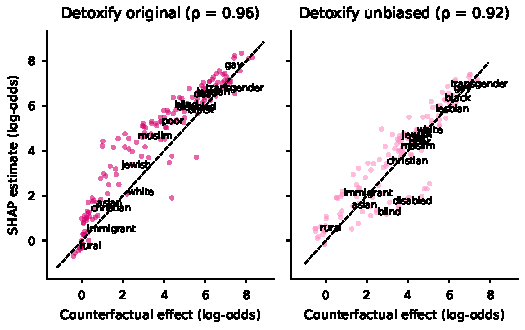
\includegraphics[width=\columnwidth]{fig_exp3_cf_vs_shap.pdf}%
}{%
  \fbox{\parbox{0.9\columnwidth}{\centering\vspace{1.5cm}Fig.~1 placeholder: copy fig\_exp3\_cf\_vs\_shap.pdf into paper/figures/\vspace{1.5cm}}}%
}
\caption{SHAP's estimate of each identity word's effect vs.\ its counterfactual effect (log-odds), one point per identity sentence ($n=150$). Dashed line: $y=x$. \todo{finalise caption}}
\label{fig:cf}
\end{figure}

% Exp 4 column changed from "MAE vs exact" to "rho vs exact": Exp 4 has no
% LIME MAE, but has rho for both explainers (exp4_summary.csv).
\begin{table}[t]
\caption{Faithfulness summary \todo{check values and finalise caption}}
\label{tab:faith}
\centering
\footnotesize
\setlength{\tabcolsep}{3pt}
\begin{tabular}{@{}lcccc@{}}
\toprule
 & $\rho$ vs.\ CF & $\rho$ vs.\ exact & Comp.\ $\uparrow$ / Suff.\ $\downarrow$ & Top word changes \\
 & (Exp 3, orig/unb) & (Exp 4, low/high) & (Exp 5, orig) & (Exp 6, 5000) \\
\midrule
SHAP   & 0.96 / 0.92 & 1.00 / 0.99 & 3.09 / $-2.43$ & n/a \\
LIME   & 0.97 / 0.97 & 1.00 / 0.98 & 3.05 / $-2.65$ & 4\% \\
Random & n/a & n/a & 0.35 / 1.30 & n/a \\
\bottomrule
\end{tabular}
\end{table}

\subsection{Deletion Test}
% Exp 5 (Bláithín). Sources: exp5_aopc.csv, exp5_aopc_by_group.csv.
% Negative sufficiency is only reported here; it is explained in Section V.
Deleting the top-ranked words lowered the toxic log-odds far more than deleting random words (Table~\ref{tab:faith}). Comprehensiveness was 3.09 for SHAP and 3.05 for LIME vs.\ 0.35 for random words with the original model, and 4.02, 4.06 and 0.95 with the unbiased model. The gap over random was largest on the Experiment~1 counter and report sentences (4.58 and 4.52 log-odds for SHAP, original model) and smallest on the control sentences, where comprehensiveness was close to zero for every explainer (SHAP $-0.02$, LIME 0.01). Sufficiency was negative for both explainers: $-2.43$ for SHAP and $-2.65$ for LIME with the original model, and $-0.97$ and $-0.85$ with the unbiased model, against $+1.30$ and $+2.63$ for random words. So keeping only the top-ranked words gave a higher toxicity score than the full sentence. The effect was strongest on report sentences ($-3.4$ for both explainers, original model).

\subsection{Where the Explainers Break}
\begin{itemize}
  \item Fig.~\ref{fig:stability} goes here. $n = 238$ sentences $\times$ 10 seeds. Sources: \texttt{exp6\_summary.csv}, \texttt{exp6\_stability\_by\_sentence.csv}, \texttt{exp6\_warning\_signs.csv}.
  \item Top word changed between seeds in 12\% of sentences at 500 samples, 4\% at 5000; mean rank stability 0.96 / 0.99.
  \item Instability vs.\ signal strength: $\rho = 0.04$ / 0.03, i.e.\ no relationship (Fig.~\ref{fig:stability} is a flat cloud, and that is the result).
  \item But fit drops on weak signals: $\rho(\text{signal}, R^2) = 0.73$; mean $R^2 \approx 0.45$ on the weakest quarter vs.\ 0.87 on the strongest; top-word agreement with SHAP 0.86 vs.\ 0.94.
  \item Warning signs for the worst 25\% of SHAP errors ($n=150$ identity sentences), AUC: SHAP--LIME disagreement 0.46, low $R^2$ 0.64, weak signal 0.80.
  \item Decide: keep Fig.~\ref{fig:stability} as is, or replot as $R^2$ vs.\ signal (EXP6 Cell 7). Caption must match either way.
\end{itemize}

\begin{figure}[t]
\centering
\IfFileExists{figures/fig_exp6_instability_vs_signal.pdf}{%
  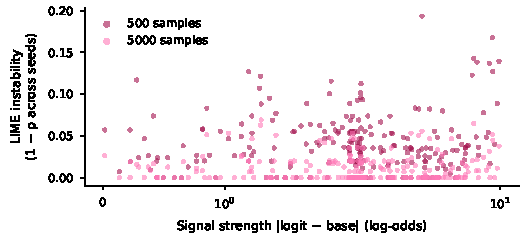
\includegraphics[width=\columnwidth]{fig_exp6_instability_vs_signal.pdf}%
}{%
  \fbox{\parbox{0.9\columnwidth}{\centering\vspace{1.5cm}Fig.~2 placeholder: copy fig\_exp6\_instability\_vs\_signal.pdf into paper/figures/\vspace{1.5cm}}}%
}
\caption{LIME instability across 10 seeds vs.\ signal strength, at 500 and 5000 samples ($n=238$ sentences). \todo{finalise caption}}
\label{fig:stability}
\end{figure}

\subsection{Sensitivity to the Removal Baseline}
\begin{itemize}
  \item 2--3 sentences with numbers. Sources: \texttt{exp3\_baselines.csv}, \texttt{exp3\_baseline\_rankings.csv}.
  \item Term ranking barely changes across dots / delete / mask: $\rho \geq 0.97$ for every pair, both models.
  \item Magnitudes do change: MAE 0.94 $\rightarrow$ 0.84 $\rightarrow$ 0.70 (original), 0.72 $\rightarrow$ 0.58 $\rightarrow$ 0.44 (unbiased); control-word $|\phi|$ (original) 0.64 $\rightarrow$ 0.43 $\rightarrow$ 0.39.
\end{itemize}
